\pdfoutput=1
\documentclass[11pt]{article}

\usepackage[margin=1in]{geometry}
\usepackage{amsmath}
\usepackage{amssymb}
\usepackage{booktabs}
\usepackage{enumitem}
\usepackage{array}
\usepackage{tikz}
\usepackage{url}
\usetikzlibrary{arrows.meta,backgrounds,fit,positioning,shapes.geometric}

\title{XScientist: A Git-Like Research Protocol for Long-Running Autonomous Scientific Discovery}

\author{
Jixiang Luo\\
\texttt{jixiangluo85@gmail.com}
}

\date{May 2026}

\begin{document}
\maketitle

\begin{center}
\textbf{Project repository:} \url{https://github.com/smileformylove/XScientist}
\end{center}

\begin{abstract}
Autonomous research systems are often evaluated as one-shot paper generators:
given a topic, they produce a manuscript and a small set of experiment logs.
This framing hides the operational problem that makes such systems difficult
to trust: research is long-running, branching, failure-prone, and dependent on
auditable handoffs between agents and humans. XScientist is a git-like
research protocol and operating system for this setting. It orchestrates idea
generation, experiment execution, manuscript drafting, self-review, repair,
quality gating, daemon scheduling, and reproducibility artifacts as one
continuously observable pipeline. The central design choice is to treat each
run as a portable research artifact rather than only as a PDF. XScientist
exports an Agent-Native Research Artifact (ARA), a protocol that records an
exploration DAG, per-node code and outputs, claim-to-evidence anchors,
content hashes, provenance, and re-execution hooks. This makes each generated
paper inspectable as a science exploration tree: failed branches, repaired
experiments, ablations, and manuscript claims remain connected to the nodes
that produced them. The system also includes deterministic integrity
forensics, sample gates, truth contracts, reviewer-oriented repair loops, and
long-running daemon controls. This paper describes the current XScientist
architecture, the ARA protocol surface, and the practical safeguards needed
to move autonomous science from single-run demos toward reproducible,
reviewable, and forkable research infrastructure. The implementation and this
manuscript source are maintained in the public GitHub repository
\url{https://github.com/smileformylove/XScientist}.
\end{abstract}

\section{Introduction}

Large language models have made it possible to automate substantial portions
of the scientific workflow: ideation, experiment scripting, result
interpretation, manuscript drafting, and review simulation
\cite{ai-scientist,ai-scientist-v2}. Related agent systems have shown that
language models can reason, act, write code, repair software, and operate
over long horizons \cite{react,reflexion,tree-of-thoughts,swe-agent,voyager}.
However, a system that generates a plausible manuscript is not necessarily a
system that can be trusted as research infrastructure. The hard problem is
not only text generation. It is the management of evidence, failures,
revisions, and handoffs over time.

XScientist addresses this operational problem. The system is designed around
four principles:

\begin{enumerate}[leftmargin=*]
  \item \textbf{Research runs should be observable.} Each stage should emit
  structured artifacts that can be inspected without replaying the entire
  workflow.
  \item \textbf{Research runs should be forkable.} A later agent should be
  able to continue from a specific experiment node instead of cold-starting
  from the final PDF.
  \item \textbf{Research claims should be grounded.} Manuscript assertions
  should remain linked to the experiment nodes and evidence artifacts that
  support them.
  \item \textbf{Research automation should expose uncertainty.} Failed
  branches, reviewer objections, integrity warnings, and blocked gates should
  be preserved as first-class outputs rather than hidden as pipeline noise.
\end{enumerate}

The result is a long-running autonomous scientific research system with a
git-like artifact protocol. XScientist can be used as a local project runner,
a continuous paper generator, or a daemon that schedules multiple research
sources over time. Its output is not just a manuscript but a structured
record of how the manuscript came to exist.

The system described here is not only a design sketch. It is tied to the
open-source XScientist repository at
\url{https://github.com/smileformylove/XScientist}, which contains the running
implementation, protocol schemas, command-line tools, examples, documentation,
and the arXiv source for this report. The repository is therefore part of the
research contribution: it is the inspectable substrate for the protocol,
figures, release workflow, and future replication attempts.

This report makes three contributions. First, it describes the design of a
long-running research operating system whose core abstractions are run
artifacts, quality gates, and operator handoffs rather than a single prompt.
Second, it specifies the ARA layer as a practical interchange format for
agent-native research state: exploration graphs, node bundles, claim anchors,
content hashes, and provenance. Third, it documents the guardrails that have
become necessary in practice, including sample-first execution, truth
contracts, deterministic integrity forensics, and daemon controls. The paper
is therefore best read as a system report and protocol proposal, not as a
claim that autonomous research can replace scientific review.

\section{Related Work}

\paragraph{Autonomous scientific discovery.}
The AI Scientist introduced an end-to-end loop for automated idea generation,
experiment execution, paper writing, and review \cite{ai-scientist}; related
open research prototypes such as autoresearch also explore lightweight
automation loops for scientific work \cite{autoresearch}. AI
Scientist-v2 extends this line with agentic tree search and workshop-level
paper generation \cite{ai-scientist-v2}. XScientist follows the same broad
goal of automating research workflows, but shifts the main abstraction from
``generate a paper'' to ``produce a forkable research protocol artifact.''
The protocol layer is intended to make continuation, review, and
cross-system handoff explicit.

\paragraph{LLM agents and long-horizon work.}
ReAct combines reasoning and acting in language models \cite{react};
Reflexion studies verbal feedback loops for language agents
\cite{reflexion}; Tree of Thoughts explores deliberate branching search
\cite{tree-of-thoughts}; Voyager demonstrates open-ended skill accumulation
in an embodied environment \cite{voyager}. Software-engineering agents such
as SWE-agent show how interface design affects autonomous repair
\cite{swe-agent}, AIDE explores code-space search for ML engineering tasks
\cite{aide}, while multi-agent frameworks such as AutoGen support
conversation-based orchestration \cite{autogen}. XScientist borrows the
branching and repair mindset of these systems but applies it to scientific
artifact management.

\paragraph{Experiment tracking and versioned research state.}
MLflow and DVC are representative tools for machine-learning lifecycle
tracking and data/model versioning \cite{mlflow,dvc}. They address important
parts of reproducibility but do not directly specify a claim-to-experiment
protocol for autonomous research manuscripts. XScientist's ARA layer is
closer to a git-like object model for research runs: a portable directory
contract with nodes, edges, content hashes, provenance, and re-execution
hooks.

\paragraph{Automated review and integrity checking.}
Reviewer-oriented systems such as DeepReviewer explore stronger automated
review signals \cite{deepreviewer}. Anti-Autoresearch motivates evidence-led
scrutiny of generated research artifacts \cite{anti-autoresearch}. XScientist
integrates reviewer-style repair with deterministic integrity forensics, but
keeps these checks conservative: they are safeguards and audit aids, not
proofs of scientific correctness.

\section{System Overview}

XScientist is organized as a research operating system. Figure
\ref{fig:pipeline} summarizes the high-level control flow. The pipeline begins
with topics or source queues, produces ranked ideas, executes experiments,
generates manuscripts, performs self-review and repair, applies quality and
integrity gates, and archives reusable artifacts.

\begin{figure}[t]
\centering
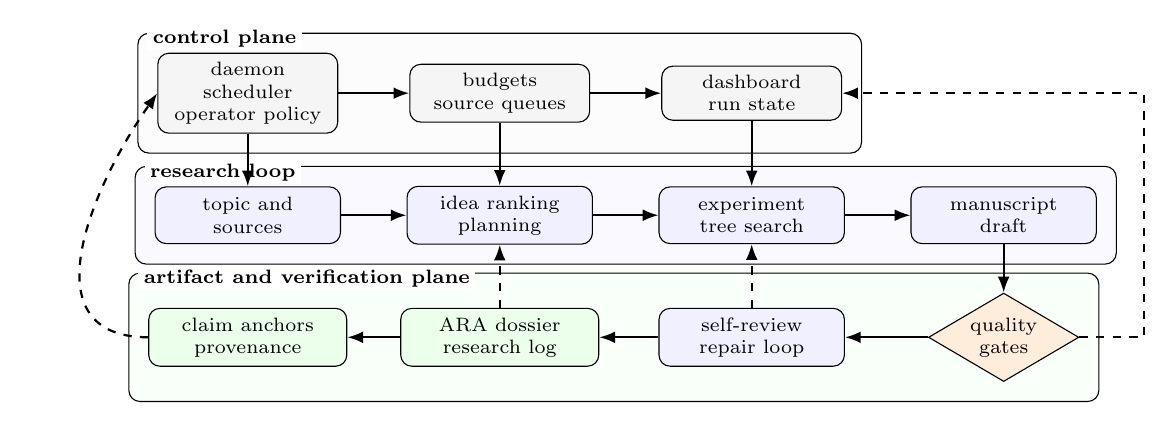
\begin{tikzpicture}[
  x=1cm,
  y=1cm,
  every node/.style={font=\scriptsize},
  lane/.style={
    draw,
    rounded corners,
    inner sep=7pt,
    fill=#1,
    fill opacity=0.13,
    text opacity=1
  },
  lane label/.style={
    font=\scriptsize\bfseries,
    anchor=west,
    fill=white,
    inner xsep=2pt,
    inner ysep=1pt
  },
  block/.style={
    draw,
    rounded corners,
    align=center,
    text width=2.12cm,
    minimum height=0.72cm,
    fill=blue!6
  },
  artifact/.style={
    draw,
    rounded corners,
    align=center,
    text width=2.28cm,
    minimum height=0.72cm,
    fill=green!8
  },
  gate/.style={
    draw,
    diamond,
    aspect=1.7,
    align=center,
    inner sep=1.1pt,
    fill=orange!14
  },
  smallblock/.style={
    draw,
    rounded corners,
    align=center,
    text width=2.05cm,
    minimum height=0.66cm,
    fill=gray!8
  },
  arrow/.style={-{Latex[length=2mm]}, thick},
  feedback/.style={-{Latex[length=2mm]}, thick, dashed}
]
\node[smallblock] (daemon) at (0,1.55) {daemon scheduler\\operator policy};
\node[smallblock] (budget) at (3.2,1.55) {budgets\\source queues};
\node[smallblock] (dash) at (6.4,1.55) {dashboard\\run state};

\node[block] (sources) at (0,0) {topic and\\sources};
\node[block] (ideas) at (3.2,0) {idea ranking\\planning};
\node[block] (experiments) at (6.4,0) {experiment\\tree search};
\node[block] (writeup) at (9.6,0) {manuscript\\draft};

\node[gate] (gates) at (9.6,-1.55) {quality\\gates};
\node[block] (review) at (6.4,-1.55) {self-review\\repair loop};
\node[artifact] (ara) at (3.2,-1.55) {ARA dossier\\research log};
\node[artifact] (claims) at (0,-1.55) {claim anchors\\provenance};

\begin{scope}[on background layer]
  \node[lane=gray!20, fit=(daemon)(budget)(dash)] (controlplane) {};
  \node[lane=blue!18, fit=(sources)(ideas)(experiments)(writeup)] (researchloop) {};
  \node[lane=green!18, fit=(claims)(ara)(review)(gates)] (artifactplane) {};
\end{scope}
\node[lane label] at ([xshift=0.12cm,yshift=-0.08cm]controlplane.north west) {control plane};
\node[lane label] at ([xshift=0.12cm,yshift=-0.08cm]researchloop.north west) {research loop};
\node[lane label] at ([xshift=0.12cm,yshift=-0.08cm]artifactplane.north west) {artifact and verification plane};

\draw[arrow] (daemon) -- (budget);
\draw[arrow] (budget) -- (dash);
\draw[arrow] (daemon.south) -- (sources.north);
\draw[arrow] (budget.south) -- (ideas.north);
\draw[arrow] (dash.south) -- (experiments.north);

\draw[arrow] (sources) -- (ideas);
\draw[arrow] (ideas) -- (experiments);
\draw[arrow] (experiments) -- (writeup);
\draw[arrow] (writeup) -- (gates);
\draw[arrow] (gates) -- (review);
\draw[arrow] (review) -- (ara);
\draw[arrow] (ara) -- (claims);

\draw[feedback] (review.north) -- (experiments.south);
\draw[feedback] (ara.north) -- (ideas.south);
\draw[feedback] (claims.west) to[out=180,in=235,looseness=1.25] (daemon.west);
\draw[feedback] (gates.east) -- ++(0.82,0) |- (dash.east);
\end{tikzpicture}
\caption{XScientist research protocol flowchart. The upper control plane
schedules sources and budgets, the middle loop performs scientific work, and
the lower artifact plane records evidence, gates, repairs, and provenance for
later audit or forked continuation. Dashed edges denote long-horizon feedback.}
\label{fig:pipeline}
\end{figure}

\subsection{Execution Modes}

The current repository exposes three main entry points.
\begin{itemize}[leftmargin=*]
  \item \texttt{run\_project.py} runs an end-to-end project from a topic or
  idea file.
  \item \texttt{continuous\_paper\_generator.py} performs batch and continuous
  generation across selected ideas and paper types.
  \item \texttt{continuous\_research\_daemon.py} runs a long-lived scheduling
  loop with source queues, dashboarding, reports, and operator controls.
\end{itemize}

\subsection{Pipeline Artifacts}

XScientist writes structured JSON and Markdown artifacts throughout the run:
idea cards, research plans, experiment registries, reviewer findings, repair
plans, manuscript candidates, quality reports, integrity forensics reports,
source provenance, and handoff briefs. These artifacts are deliberately more
important than transient console output. They give downstream agents and
human operators a stable interface for audit and continuation.

\subsection{Core Components}

The system is decomposed into components that can be used independently or as
part of the full pipeline.

\paragraph{Ideation and planning.}
The ideation layer converts topics and source queues into candidate ideas,
rankings, and research plans. Plans contain tasks, expected outputs,
acceptance checks, baselines, and execution policy hints. In high-quality
runs, the planner also produces artifacts used by later quality and truth
checks.

\paragraph{Experiment execution.}
Experiments are executed through a tree-search-style loop that records code,
stdout/stderr, metrics, plots, and failure states. XScientist treats failed
branches as useful evidence: they may explain why a later repair exists, why a
claim was softened, or why a branch should not be continued.

\paragraph{Writing and review.}
The writing layer produces LaTeX manuscripts and structured metadata. The
review layer applies text and figure review, extracts issues, schedules repair
actions, and can run multiple reviewer-oriented strategies such as novelty,
rigor, clarity, and reproducibility checks.

\paragraph{Indexing and management.}
The management layer surfaces boards for generated papers, review issues,
repair priorities, process alignment, and evolution signals. This keeps the
system usable as an operating workflow rather than only as a batch script.

\subsection{Operating Assumptions}

XScientist assumes that autonomous research should be operated under explicit
budgets and review boundaries. The system can run for long periods, but it
does not assume that every cycle should advance to a full manuscript. A run
may stop because a sample gate fails, because a truth contract is violated,
because integrity forensics finds hard flags, or because the operator pauses
the daemon. These stopping states are treated as valid outcomes.

\section{Agent-Native Research Artifacts}

The most important interface in XScientist is the Agent-Native Research
Artifact (ARA). An ARA is a directory rooted at a \texttt{manifest.json} file
and an \texttt{exploration\_graph.json} file. It is designed to be read by
another agent without requiring that agent to reverse-engineer the final
paper.

\subsection{Exploration DAG}

Each ARA stores an exploration DAG whose nodes represent concrete experiment,
repair, failure, ablation, or manuscript-candidate states. Edges encode the
parent-to-child evolution of the research process. The system validates that
the graph is directed and acyclic, writes a summary file, and can render a
self-contained HTML visualization. This turns each paper into a science
exploration tree.

The exploration tree is intentionally not a polished success-only lineage.
It includes bug states, discarded branches, and repaired branches because
those states are often the most important for later review. A downstream agent
that sees only the final successful experiment cannot know whether the result
was robust, whether a metric was changed midstream, or whether a failed
baseline was silently dropped. ARA makes those transitions inspectable.

\begin{figure}[t]
\centering
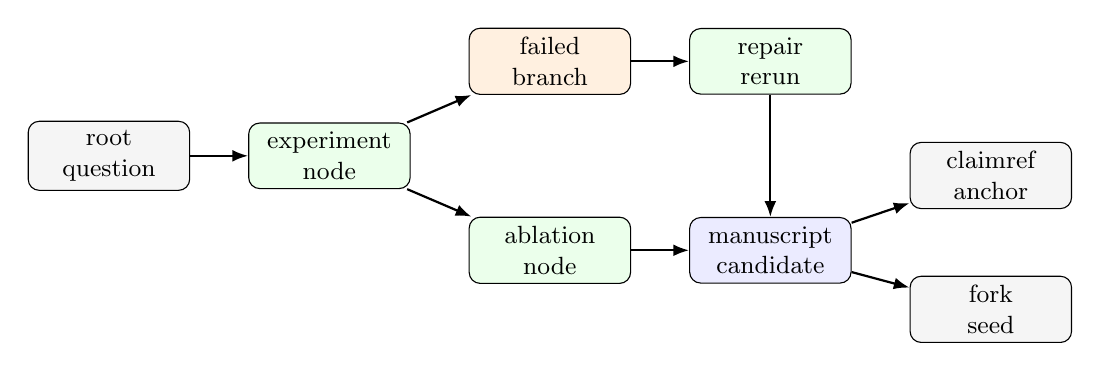
\begin{tikzpicture}[
  x=1cm,
  y=1cm,
  every node/.style={font=\small},
  state/.style={
    draw,
    rounded corners,
    align=center,
    minimum width=2.05cm,
    minimum height=0.78cm,
    fill=gray!8
  },
  good/.style={state, fill=green!8},
  warn/.style={state, fill=orange!12},
  paper/.style={state, fill=blue!8},
  arrow/.style={-{Latex[length=2mm]}, thick}
]
\node[state] (root) at (0,0) {root\\question};
\node[good] (exp) at (2.8,0) {experiment\\node};
\node[warn] (fail) at (5.6,1.2) {failed\\branch};
\node[good] (repair) at (8.4,1.2) {repair\\rerun};
\node[good] (ablate) at (5.6,-1.2) {ablation\\node};
\node[paper] (candidate) at (8.4,-1.2) {manuscript\\candidate};
\node[state] (claim) at (11.2,-0.25) {claimref\\anchor};
\node[state] (fork) at (11.2,-1.95) {fork\\seed};

\draw[arrow] (root) -- (exp);
\draw[arrow] (exp) -- (fail);
\draw[arrow] (fail) -- (repair);
\draw[arrow] (repair) -- (candidate);
\draw[arrow] (exp) -- (ablate);
\draw[arrow] (ablate) -- (candidate);
\draw[arrow] (candidate) -- (claim);
\draw[arrow] (candidate) -- (fork);
\end{tikzpicture}
\caption{Conceptual science exploration tree. ARA preserves both successful
and failed branches, allowing later agents to audit or fork a specific node.}
\label{fig:tree}
\end{figure}

\subsection{Content Hashing and Provenance}

ARA uses content hashes to identify node payloads and manifest revisions.
Hashes are computed over canonical payloads such as code, metrics, and
optional provenance fields. Forked runs preserve parent pointers, so a child
research run can describe which previous ARA and node seeded it. The protocol
therefore behaves like a lightweight object model for research state.

In practice, this gives XScientist a commit-like substrate. The final PDF is
only one rendered view. The underlying research state can be diffed, logged,
forked, or frozen. When an ARA is committed to a normal git repository, git
records file-level snapshots, while ARA commands expose node-level scientific
history inside those snapshots.

\subsection{Claim Anchoring}

The writing stage can insert invisible \texttt{\textbackslash claimref}
markers after quantitative or evidence-sensitive claims. A claim registry
scans the manuscript source and writes claim records under the ARA. This
creates a two-way link between paper assertions and the experiment nodes that
support them. Claim coverage can then be summarized and used by quality gates
or downstream reviewers.

\subsection{Fork, Diff, Log, and Verify}

The companion CLI \texttt{run\_ara\_fork.py} exposes operational verbs:
\texttt{inspect}, \texttt{exec}, \texttt{fork}, \texttt{freeze},
\texttt{validate}, \texttt{verify}, \texttt{diff}, \texttt{log}, and
\texttt{refs}. These commands let an operator inspect a node, re-execute its
code, create a new seed ARA, compare two ARAs, or walk the provenance chain.
The same graph data underlies the HTML visualization, the log view, and
node-level diffs.

\subsection{ARA Directory Contract}

The minimal ARA contract requires two files: \texttt{manifest.json} and
\texttt{exploration\_graph.json}. Optional but common files include per-node
\texttt{code.py}, \texttt{term\_out.log}, \texttt{metrics.json},
\texttt{plots.json}, environment snapshots, claim records, verification
reports, repair history, Pareto candidate pools, and a human-facing HTML graph
view. Missing artifacts are not treated as fatal if they are declared; this
lets lightweight producers implement the protocol incrementally while still
being consumable by stricter tools.

\begin{table}[t]
\centering
\small
\begin{tabular}{p{0.23\linewidth}p{0.18\linewidth}p{0.49\linewidth}}
\toprule
Artifact & Status & Purpose \\
\midrule
\texttt{manifest.json} & required & Entry point, schema version, counts,
references, provenance, and missing-artifact declarations. \\
\texttt{exploration\_}\linebreak\texttt{graph.json} & required & Node and edge set for the
science exploration DAG. \\
\texttt{nodes/<id>/} & optional & Per-node code, metrics, logs, plots,
environment descriptors, and rerun script. \\
\texttt{claims/} & optional & Claim-to-node anchors extracted from manuscript
source. \\
\texttt{verify/} & optional & Re-execution reports and metric-drift checks. \\
\texttt{pipeline/} & optional & Mirrored planning, review, repair, and gate
artifacts for downstream agents. \\
\bottomrule
\end{tabular}
\normalsize
\caption{Simplified ARA directory contract. The protocol is file-based so it
can be archived, diffed, copied, or consumed by non-XScientist tools.}
\label{tab:ara-contract}
\end{table}

\subsection{Why a Protocol Instead of a Database}

A database would make local querying convenient but would make handoff harder.
ARA uses ordinary files so that artifacts can be copied, archived, attached to
issues, reviewed in pull requests, or consumed by other agents without running
a XScientist service. This design is deliberately close to how software
engineering uses repositories: the protocol specifies what must exist on
disk, while different tools can provide richer user interfaces over the same
state.

\section{Quality and Integrity Controls}

Autonomous research systems require checks that are deterministic enough to
be run in CI and explicit enough to be audited later. XScientist implements
several such controls.

\subsection{Self-Review and Repair}

The self-review subsystem runs LLM-based and VLM-assisted reviews, extracts
structured issues, prioritizes repairs, and records repair attempts. The
system tracks whether reviewer objections were addressed, whether manuscript
changes regressed earlier claims, and whether quality thresholds were met.

Repair is represented as a trace rather than as a single overwrite. The
system records which issue motivated a repair, which artifact was modified,
which checks were rerun, and whether the repair introduced new risks. This is
important for generated manuscripts because a fluent rewrite can hide evidence
loss. XScientist therefore treats repair coverage and regression detection as
first-class quality signals.

\subsection{Truth Contracts}

Truth contracts translate a research plan into explicit constraints. They
separate objective facts, comparability constraints, artifact-binding rules,
branch-state rules, and value guardrails. For example, a manuscript should not
claim a baseline-comparable improvement unless the experiment registry
contains a completed run on the declared dataset, metric, and baseline.

The categories are intentionally broad: objective facts, comparability
constraints, artifact-binding rules, branch-state transitions, and value
guardrails. They are not a formal proof system. They are a pragmatic checklist
that converts ambiguous planner intent into concrete conditions that can be
checked later by gates, reviewers, or downstream agents.

\subsection{Sample Gates}

Before full generation, sample gates can require that a small planned task
has a completed experiment record, a budget audit, passing acceptance checks,
and a result summary. This prevents the system from scaling a flawed plan into
a full paper when the cheap preliminary evidence is missing.

\subsection{Deterministic Integrity Forensics}

XScientist adapts an evidence-ledger pattern inspired by
Anti-Autoresearch into the manuscript stage. The integrity forensics pass is
not an authorship detector. It builds a span-anchored ledger from the
manuscript source, applies model-free consistency checks, and writes a
deterministic adjudication report. Hard findings can block submission-ready
status; soft findings are reported for reviewer attention.

The deterministic design is deliberate. Model-based critique is useful, but a
submission gate needs repeatable behavior. Integrity forensics therefore
focuses on checks that can be rerun with the same result: suspicious pipeline
artifacts in the manuscript, unsupported strong wording, arithmetic drift in
reported deltas, citation placeholders, repeated caption/table presentation
signals, and evidence-ledger gaps. It is a conservative screen for risks that
deserve attention before a paper is treated as submission-ready.

\subsection{Decision Logs and Gate Preconditions}

Recent XScientist runs also write decision logs for workflow strategy,
sample-gate outcomes, and model-provider choices. Gate preconditions are
checked before expensive or high-risk stages proceed. For example, a quality
gate that requires high-quality mode should not run under a cheaper classic
pipeline by accident; a full-generation stage should not proceed when the
sample gate is blocked. These checks turn implicit workflow assumptions into
explicit runtime contracts.

\begin{table}[t]
\centering
\small
\begin{tabular}{p{0.25\linewidth}p{0.33\linewidth}p{0.32\linewidth}}
\toprule
Control & Signal & Effect \\
\midrule
Sample gate & Sample task completion, budget audit, acceptance checks &
Blocks full generation when cheap preliminary evidence is absent. \\
Truth contract & Plan-derived facts, comparability rules, artifact bindings &
Prevents unsupported or mismatched claims from being treated as ready. \\
Integrity forensics & Span ledger, deterministic consistency checks & Raises
hard or soft manuscript risk flags. \\
Review repair trace & Structured issues, repair attempts, regression checks &
Shows how reviewer objections were addressed. \\
Gate preconditions & Workflow mode, quality mode, gate requirements & Stops
incompatible stage combinations before expensive execution. \\
\bottomrule
\end{tabular}
\normalsize
\caption{Quality controls in XScientist. The goal is not to prove correctness
automatically, but to make risk states explicit and reproducible.}
\label{tab:quality-controls}
\end{table}

\section{Long-Running Daemon Operation}

The daemon mode treats research as an ongoing operation rather than a single
script invocation. It supports source queues, source health tracking,
dashboard serving, daily reports, handoff briefs, pause/resume controls,
source boosting and cooldown, failure protection, and strategy feedback.

This matters because autonomous research systems accumulate operational
state. A topic source may produce weak ideas for a week and then recover. A
review-hardening source may be valuable only after enough experimental
evidence exists. XScientist therefore records source-level and portfolio-level
signals so later cycles can adjust scheduling rather than replay a fixed
script.

\subsection{Operator Controls}

The daemon is designed for supervised autonomy. Operators can pause and
resume, stop after the current cycle, force or boost a source, apply a
cooldown, inspect dashboard state, and generate handoff reports. This makes
the system suitable for long-running local operation where full automation is
not always desirable. A useful autonomous research system should make it easy
to interrupt, inspect, and redirect.

\subsection{Feedback Loops}

The daemon collects feedback at several levels: paper-level quality signals,
source-level health, strategy-level success rates, repair pressure, and
process alignment. These signals can influence later scheduling and execution
policy. For example, a source that repeatedly produces blocked sample gates
can be cooled down, while a source producing useful review-hardening tasks can
be boosted when a manuscript is near submission.

\section{Reproducibility and Release Workflow}

XScientist separates source code from generated research outputs by default.
Runtime artifacts are written outside the repository unless the operator
chooses otherwise. This reduces accidental repository pollution while keeping
outputs easy to archive. For reproducibility, a report should cite the
public repository, the exact commit hash, configuration, model choices, output
directory, and the ARA root used for any generated paper. For the present
system report, the canonical repository is
\url{https://github.com/smileformylove/XScientist}.

The recommended release workflow for a generated manuscript is:
\begin{enumerate}[leftmargin=*]
  \item run the project or daemon under an explicit output root and budget;
  \item inspect the generated manuscript, ARA, review reports, and integrity
  forensics;
  \item verify or re-execute important ARA nodes where feasible;
  \item check claim coverage and manually review evidence-sensitive claims;
  \item package the manuscript and artifact references with commit hashes.
\end{enumerate}

This workflow does not guarantee correctness, but it raises the cost of
silent evidence loss and makes later review more concrete.

\section{Comparison to One-Shot Paper Generation}

Table \ref{tab:comparison} contrasts the XScientist design with a typical
one-shot autonomous paper generator.

\begin{table}[t]
\centering
\begin{tabular}{p{0.29\linewidth}p{0.29\linewidth}p{0.32\linewidth}}
\toprule
Dimension & One-shot generator & XScientist \\
\midrule
Primary output & PDF or draft & PDF plus structured research artifact \\
Failure handling & Often discarded & Preserved as DAG branches \\
Continuation & Prompt-level restart & Node-level fork from ARA \\
Claim grounding & Implicit in prose & Explicit claim-to-node anchors \\
Review & Text feedback & Structured issues, repair attempts, gates \\
Operations & Manual reruns & Daemon, reports, dashboard, controls \\
\bottomrule
\end{tabular}
\caption{Design contrast between one-shot generation and XScientist's
artifact-centered workflow.}
\label{tab:comparison}
\end{table}

\section{Evaluation Strategy}

This report does not present a large benchmark claiming that XScientist
outperforms other autonomous research systems. Instead, the current evaluation
strategy is artifact-centered. A run should be judged by whether it produces:

\begin{itemize}[leftmargin=*]
  \item a valid ARA with a DAG exploration graph;
  \item per-node code, metrics, logs, and environment descriptors when
  available;
  \item claim anchors and claim coverage summaries for evidence-sensitive
  manuscript statements;
  \item review and repair artifacts that explain how manuscript changes were
  made;
  \item deterministic integrity reports with clear hard and soft findings;
  \item enough provenance for another agent or human to fork, verify, or
  reject the result.
\end{itemize}

This evaluation style is closer to systems engineering than to leaderboard
scoring. It asks whether the research process is inspectable and recoverable.
Future empirical work should compare ARA-backed continuation against cold
start baselines, measure the cost of re-execution, and study whether
claim-anchored review improves human error detection.

\section{Limitations}

XScientist does not make autonomous research automatically correct. The
system can organize evidence, preserve provenance, and expose warnings, but
human review remains necessary for scientific validity, ethical judgment, and
final submission decisions. The current system also has several engineering
limitations:

\begin{itemize}[leftmargin=*]
  \item Re-execution can be expensive or environment-dependent when nodes
  call external APIs, GPUs, or web services.
  \item Integrity forensics is deterministic but incomplete; it catches some
  classes of inconsistency and overclaiming, not all scientific errors.
  \item ARA is a protocol surface rather than a universal standard; broader
  adoption requires independent producers and consumers.
  \item The daemon improves operations, but long-running autonomy still needs
  explicit budgets, stop conditions, and operator oversight.
  \item The present paper is a system report. It documents the implementation
  and protocol surface but does not yet provide a controlled user study or a
  broad external benchmark.
\end{itemize}

\section{Ethical and Safety Considerations}

Autonomous research tooling can create plausible but incorrect scientific
artifacts at high speed. XScientist is therefore designed to preserve
uncertainty, not to erase it. The system records failed branches, exposes
blocked gates, and explicitly states that integrity forensics is incomplete.
Users should not submit generated papers without human review, should disclose
substantial automated assistance when appropriate, and should avoid using the
system for domains where erroneous claims can cause direct harm without
additional expert oversight.

There is also an operational safety concern: long-running agents can consume
API credits, compute, and storage unexpectedly. XScientist includes output
isolation, preflight checks, daemon controls, and budget-oriented gates, but
operators remain responsible for configuring limits and monitoring runs.

\section{Discussion}

The central claim of XScientist is that autonomous research should be judged
not only by the final manuscript but by the quality of the artifact trail that
produced it. A generated paper without a recoverable experiment tree is hard
to audit. A failed branch without provenance is hard to learn from. A claim
without a node anchor is hard to verify. XScientist makes these relations
first-class.

The same design suggests a path toward collaborative autonomous science:
systems can exchange ARAs, fork one another's nodes, verify claims without
parsing PDFs, and use git-like diffs to review scientific changes. This does
not remove the need for human scientists. It gives human reviewers and
downstream agents a stronger substrate to inspect.

\section{Conclusion}

XScientist is a long-running autonomous scientific research system built
around structured artifacts, continuous operation, and a git-like research
protocol. Its ARA export turns each paper into a science exploration tree with
claim anchors, content hashes, provenance, and re-execution hooks. Together
with self-review, repair loops, sample gates, truth contracts, deterministic
integrity forensics, and daemon scheduling, this design moves autonomous
research from one-shot paper generation toward reproducible and forkable
research infrastructure.

\section*{Availability}

The primary artifact for this report is the public XScientist GitHub
repository:
\begin{center}
\url{https://github.com/smileformylove/XScientist}
\end{center}
It contains the implementation, ARA protocol schemas, command-line tools,
examples, documentation, and tests. The arXiv source for this system report is
maintained in the same repository under:
\begin{center}
\texttt{paper/xscientist\_arxiv/}
\end{center}
Reproducibility claims should cite both the repository URL and the exact commit
hash used to run or inspect the system.

\section*{Acknowledgements}

XScientist builds on ideas from AI Scientist, autoresearch, AIDE,
DeepReviewer, and related open-source autonomous research and review systems.
The integrity forensics layer adapts an evidence-ledger pattern inspired by
Anti-Autoresearch.

\begin{thebibliography}{99}

\bibitem{ai-scientist}
Chris Lu, Cong Lu, Robert Tjarko Lange, Jakob Foerster, Jeff Clune, and David Ha.
\newblock The AI Scientist: Towards Fully Automated Open-Ended Scientific Discovery.
\newblock arXiv preprint arXiv:2408.06292, 2024.

\bibitem{ai-scientist-v2}
Yutaro Yamada, Robert Tjarko Lange, Cong Lu, Shengran Hu, Chris Lu, Jakob Foerster, Jeff Clune, and David Ha.
\newblock The AI Scientist-v2: Workshop-Level Automated Scientific Discovery via Agentic Tree Search.
\newblock arXiv preprint arXiv:2504.08066, 2025.

\bibitem{autoresearch}
Andrej Karpathy.
\newblock autoresearch.
\newblock \url{https://github.com/karpathy/autoresearch}.

\bibitem{aide}
WecoAI.
\newblock AIDE: AI-Driven Exploration in the Space of Code.
\newblock \url{https://github.com/WecoAI/aideml}.

\bibitem{react}
Shunyu Yao, Jeffrey Zhao, Dian Yu, Nan Du, Izhak Shafran, Karthik Narasimhan, and Yuan Cao.
\newblock ReAct: Synergizing Reasoning and Acting in Language Models.
\newblock In \emph{International Conference on Learning Representations}, 2023.

\bibitem{reflexion}
Noah Shinn, Federico Cassano, Edward Berman, Ashwin Gopinath, Karthik Narasimhan, and Shunyu Yao.
\newblock Reflexion: Language Agents with Verbal Reinforcement Learning.
\newblock In \emph{Advances in Neural Information Processing Systems}, 2023.

\bibitem{tree-of-thoughts}
Shunyu Yao, Dian Yu, Jeffrey Zhao, Izhak Shafran, Thomas L. Griffiths, Yuan Cao, and Karthik Narasimhan.
\newblock Tree of Thoughts: Deliberate Problem Solving with Large Language Models.
\newblock In \emph{Advances in Neural Information Processing Systems}, 2023.

\bibitem{swe-agent}
John Yang, Carlos E. Jimenez, Alexander Wettig, Kilian Lieret, Shunyu Yao, Karthik Narasimhan, and Ofir Press.
\newblock SWE-agent: Agent-Computer Interfaces Enable Automated Software Engineering.
\newblock arXiv preprint arXiv:2405.15793, 2024.

\bibitem{autogen}
Qingyun Wu et al.
\newblock AutoGen: Enabling Next-Gen LLM Applications via Multi-Agent Conversation.
\newblock arXiv preprint arXiv:2308.08155, 2023.

\bibitem{voyager}
Guanzhi Wang, Yuqi Xie, Yunfan Jiang, Ajay Mandlekar, Chaowei Xiao, Yuke Zhu, Linxi Fan, and Anima Anandkumar.
\newblock Voyager: An Open-Ended Embodied Agent with Large Language Models.
\newblock arXiv preprint arXiv:2305.16291, 2023.

\bibitem{mlflow}
Matei Zaharia et al.
\newblock Accelerating the Machine Learning Lifecycle with MLflow.
\newblock IEEE Data Engineering Bulletin, 2018.

\bibitem{dvc}
Dmitry Petrov, Pavel Gritsenko, Daniil Vorobev, and Ivan Isakov.
\newblock Data Version Control: Data and Model Management for Machine Learning.
\newblock \url{https://dvc.org}.

\bibitem{deepreviewer}
ResearAI.
\newblock DeepReviewer-v2.
\newblock \url{https://github.com/ResearAI/DeepReviewer-v2}.

\bibitem{anti-autoresearch}
wanshuiyin.
\newblock Anti-Autoresearch.
\newblock \url{https://github.com/wanshuiyin/Anti-Autoresearch}.

\end{thebibliography}

\end{document}
